\setcounter{page}{1}
\chapter{Theory}
The main measurement principle of a microfluidic channel in connection with a \gls{gmr}-Sensor has been already described and characterized exhaustively by \citet{lit:thes:helou}, \citet{lit:thes:reisbeck} and others. \cite{lit:thes:esthi,lit:thes:brenner} Therefore, this theoretical part will focus on (bio-)physical aspects of a cell rolling motion inside a microfluidic channel and surface modification chemistry.

\section{Microfluidics}

\subsection{Incompressibility of Fluid Flows}

The main experiments of this work were carried out in microfluidic environments, which exhibit favorable properties compared to common macrofluidic systems. From a fluid-mechanical standpoint, shrinking the scales makes interfacial as well as electrokinetic phenomena much more significant, and reduces the importance of pressure and gravity.\cite{lit:fluidic:kirby} However, electrodynamics, chemistry and fluid dynamics are incetricably intertwined, so that fluid flow can create electric fields (and vice versa), with a degree of coupling driven by the surface chemistry. Many of the resulting phenomena arise or can be explained by the conservation of mass described by the continuity equation (Eq. \ref{eq:continuityM}) and the conservation of momentum described by the Cauchy-Momentum equation (eq. \ref{eq:cauchymomentum}) and the resulting Navier-Stokes equation(eq. \ref{eq:navierstokes}).

\begin{align}
	\frac{\partial}{\partial t} \iiint \rho \ \mathrm{dV} &= - \iint \rho \mathbf{u} \cdot \vv{n} \ \mathrm{dA} \label{eq:continuityM}\\
	\nabla \cdot \mathbf{u} &= 0 \label{eq:conservMass}\\	
	\frac{\partial}{\partial t} \iiint \rho\mathbf{u} \ \mathrm{dV} &= - \iint \rho \mathbf{u}\mathbf{u} \cdot \vv{n} \ \mathrm{dA} + \iint \boldsymbol{\tau} \cdot \vv{n} \ \mathrm{dA}  + \iiint  \sum_{i}\mathbf{f}_i \ \mathrm{dV} \label{eq:continuityP} \\	
		\rho \frac{\partial \mathbf{u}}{\partial t} + \rho\mathbf{u} \cdot \nabla \mathbf{u} &= \nabla \cdot \boldsymbol{\tau} + \sum_{i}\mathbf{f}_i \label{eq:cauchymomentum} \\			
\end{align}
The foremost assumption in fluid dynamics is termed ``incompressibility'', when density gradients are negligibly small to assume a uniformity thereof. This leads to a significant simplification of the conservation equations, because any transfer from kinetic to internal energy can be ignored.\footnote{For sake of completeness, it should be mentioned that viscous forces can also transfer energy irreversibly to internal energy. However, they are inversely proportional to the system's size, and hence omitted.}
%This first premise simplifies the continuity equation.
This equation states that the mass of a control volume (in this case the volume integral over the \gls{rho}) can only change by the mass flux over its \gls{surfnormal} transported by the \gls{u}. For constant \gls{rho} the mass does never change over time. This finding and the application of Gauss's theorem yields the conservation of mass in an incompressible fluid. (Eq. \ref{eq:conservMass})


\subsection{Flow and Shear in Microchannels with Viscous Fluids}

The final equation and Gauss's theorem can now be applied to the conservation of momentum relation. (Eq. \ref{eq:continuityP}) Integration yields then the Cauchy momentum equation which states that any change in momentum inside a control volume ($\rho \frac{\partial \mathbf{u}}{\partial t}$) is caused by convective transport for or to the volume ($\rho\mathbf{u} \cdot \nabla \mathbf{u}$), surface stresses ($ \nabla \cdot \boldsymbol{\tau}$), and the volumetric net body forces ($\mathbf{f}_i$) such as gravity or electrostatics.

Hereby, the surface stress \gls{tau} can be further decomposed into the \gls{tau_p} and \gls{tau_v} as shown in the equations \ref{eq:surfaceStressTensor}. Characteristically, the pressure related contributions act normal and independently from \gls{u} whereas viscous forces act normal and tangential, and are dependent on \gls{u}. The \gls{tau_p} can therefore be expressed by a scalar pressure acting in every spatial dimension which is spanned by the identity. 

The viscous stresses however can not be described by a continuum equation but only by a constitutive relation of atomistic processes. The underlying fundamental model of Newton's mechanics assumes that \gls{eta} is neither dependent on any velocity nor on the strain rate. Therefor, fluids which satisfy this condition are called ``Newtonian fluids''. Omitting special cases such as shear-thinning, -thickening or complex colloidal fluids such as undilute blood, \gls{eta} is the scalar proportionality that relates the strain rate to surface stress.\cite{lit:fluidic:kirby} This is captured in the equation $\boldsymbol{\tau}_{viscous} = 2\eta \mathbf{\epsilon} $. Thereby, \gls{epsilon} is part of the decomposition of an unidirectional flow field. It resembles on the one hand side any stretching or squeezing of fluid by ``extensional'' strain and on the other hand side ``shear'' strain which is responsible for skewing. \cite{lit:fluidic:kirby}
\begin{align}
	\boldsymbol{\tau} &= \boldsymbol{\tau}_{viscous} +  \boldsymbol{\tau}_{pressure} = 2\eta \boldsymbol{\epsilon} - p \mathbf{I}_{\scaleto{3 \times 3}{4pt}} \label{eq:surfaceStressTensor}\\
	\nabla \cdot \boldsymbol{\tau}_{viscous} &= \nabla \cdot 2\eta \boldsymbol{\epsilon} = \nabla \cdot \eta \nabla \mathbf{u} \ \underset{uniform}{\overset{only \ if \ \eta}{=}} \ \eta \nabla^2 \mathbf{u} 	\label{eq:divergence_Stresstensor} \\
	\aunderbrace{\vphantom{\sum_{i}} \rho \frac{\partial \mathbf{u}}{\partial t}}_{\mathrm{Transient}} + \aunderbrace{\vphantom{\sum_{i}}\rho\mathbf{u} \cdot \nabla \mathbf{u}}_{\mathrm{Convection}} &= \aunderbrace{\vphantom{\sum_{i}}-\nabla p}_{\mathrm{Pressure}} + \aunderbrace{\vphantom{\sum_{i}}\eta \nabla^2 \mathbf{u}}_{\mathrm{Viscous}} + \aunderbrace{\sum_{i}\mathbf{f}_i}_{\mathrm{Body \ Forces}} \label{eq:navierstokes}
\end{align}
The divergence of \gls{tau_v}, as used in the incompressible Cauchy momentum equation (Eq. \ref{eq:cauchymomentum}), can then be simplified with Eq. \ref{eq:divergence_Stresstensor} further by taking advantage of the anti-transpose symmetry of the flow field. If \gls{eta} is also uniform respectively isotropic across the channel, the divergence is completely independent of the scalar viscosity.  Applying all assumptions to the Cauchy momentum equation (Eq. \ref{eq:cauchymomentum}) yields as final result the \gls{nse}. (Eq. \ref{eq:navierstokes}) 

However, the \gls{nse} has no analytic solution yet and can in consequence only solve defined boundary problems. The two most common boundary conditions herefore are the ``no-penetration condition'' ($\mathbf{u} \cdot \vv{n} = 0$) and the ``no-slip condition'' ($\mathbf{u}_t = \mathbf{u} - (\mathbf{u}\cdot \vv{n}) \vv{n} = 0$), which state that the normal and tangential components of fluid velocity are per definition zero at motionless, impermeable walls.\newline
Besides these conditions, many problems arise due to turbulent flow and therefor transient effects. Mathematically, this can be avoided by simply neglecting the time-dependent term in the \gls{nse}. Also, it can be argumented from a systematic point of view that, for viscosity-dominated flows, fluid moves in isoplanar ``lamina''. In experimental observations, these laminar flows then proved to be stable to perturbations thus steady.

\begin{equation}
	\mathit{Re}\ =\ \frac{\mathrm{\mathsf{fluid\ density\ \cdot\ velocity\ \cdot\ size}}}{\mathrm{\mathsf{viscosity}}} \label{eq:reynolds}
\end{equation}

In a first order approximation, the dimensionless \gls{re}, which compares the inertia to viscous forces, allows a qualitative prognosis about the flow regime. (Eq. \ref{eq:reynolds}) If it results below a threshold of 2300, laminar flow can be assumed in Hagen-Poiseuille flows. This holds true for the utilized microfluidic with the dimensions \SI{12000}{\micro\meter} x \SI{700}{\micro\meter} x \SI{150}{\micro\meter} (l x w x h) and aequous buffer solutions, where the channel width considered as characteristic length $l$. Hence, several fluidic phenomena such as deterministic pathlines as well as simplifications of the \gls{nse} can be exploited in the present system. 

In the model case of a flow through a rectangular channel, no analytical solution of the \gls{nse} exists, but a Fourier Series expansion if the width is larger than height of a channel as shown in \citet{lit:fluidic:bruus}.\footnote{The equation \ref{eq:flowVelocityRect} shows that height deviations can have prominent influence on a channel velocity simulation as it is proportional to $h^2$. Further, the flow rate depends even on $h^3$.} 
Equation \ref{eq:flowVelocityRect} determines the magnitude of the flow field parallel to the pressure gradient in relation to the horizontal dimension $y$ and vertical dimension $z$ with respect to the channel dimensions height $h$ and width $w$. An integration over the flow field in the channel cross section yields the \gls{q}. (Eq. \ref{eq:flowRateRect})

  \begin{align}
\mathbf{u}   _x(y,z) &= \frac{4 h^2 \Delta p}{\pi^3 \eta l} \sum_{n,odd}^{\infty} \frac{1}{n^3} \left( 1- \frac{\cosh (n \pi \frac{y}{h})}{\cosh (n \pi \frac{w}{2h})} \right) \sin (n \pi \frac{z}{h}) \label{eq:flowVelocityRect} \\
  Q    &= \int_{-\frac{1}{2}w}^{\frac{1}{2}w} \int_{0}^{h} u   _x(y,z) \ \mathrm{dzdy} \approx \frac{h^3 w \Delta p}{12 \eta l} \left( 1 - \frac{h}{w}) \right) \label{eq:flowRateRect} \mathrm{, \ for \ } h < w
\end{align}


\subsection{Force Equilibrium of Microbeads}
Although microfluidic systems mostly operate in a low inertia regimes as specified by low \gls{re}, the force equilibrium and subsequently the velocity of any particle in the fluid stream is influenced as it moves closer to the boundaries. Therefore, a short overview over all acting forces shall be given here.


\begin{align}
	\mathbf{F}_{drag,wall} &= -6 \pi \eta r \ \overline{\mathbf{u}} \ K \label{eq:f:drag}\\
	K &=  \frac{4}{3} \sinh \alpha \sum_{n=0}^{\infty} \left(\frac{n(n+1)}{(2n-1)(2n+3)} \ \cdot \ A \right) \label{eq:f:wall-correction}\\
	\alpha &= \cosh^{-1}\frac{z}{r} \\
	A &= \left(\frac{2 \sinh((2n+1)\alpha) + (2n+1)\sinh2\alpha}{(2\sinh((n+0.5)\alpha))^2 -((2n+1)\sinh\alpha)^2 }-1\right)\\
	K_{approx} &= \frac{24}{\mathit{Re}} *\left(\frac{1+\frac{2\eta_{fluid}}{3 \eta_{particle}}}{1+\frac{\eta_{fluid}}{ \eta_{particle}}}\right) \label{eq:correctionApprox}\\
	v_z &= \frac{3}{64} \mathit{Re}_s u_s \ = \ \frac{3}{64} \frac{\rho_{fluid} r u_s}{\eta} u_s \ , \ (\frac{\rho_{fluid} l_w u_s}{\eta}) \ll 1\label{eq:repulsion_v}\\
	\mathbf{F}_{buoyancy} &= -\frac{4}{3}\pi r^3 \ \rho_{fluid} \ g \label{eq:f:buoyancy}\\
	\mathbf{F}_{gravity} &= +\frac{4}{3}\pi r^3 \ \rho_{particle} \ g \label{eq:f:grav}\\
	\mathbf{F}_{shear} &= \frac{81.2}{4} (\mathbf{u} - u_p) r^2 \sqrt{\frac{\rho_{fluid}}{\eta} \nabla \mathbf{u}} \\
	\mathbf{F}_{magnus} &=  \frac{1}{8}\pi r^3 \rho_{fluid} \ ( \mathbf{u} \times \mathbf{\Omega} )\\
	\sum_{i} \mathbf{F} &\overset{!}{=} 0 \\
	\omega &= \frac{0.025r \mathbf{u}}{l^2(1-0.6526\frac{r}{l})} \mathrm{, \ for \ } (\frac{r}{l})^2 \ll 1	
\end{align}

\subsubsection{Stoke's Drag}
The foremost force to move particles inside a microfluidic channel is \gls{f:drag}.(Eq. \ref{eq:f:drag}) It originates in the viscous fluid moving past the sphere surface, where a slip condition has to be applied. The fluid therefor has to displace its elements in front of the movement direction of a particle. \cite{lit:fluidic:motion_sphere_to_plane_surface} 
In the vertical dimension with a channel wall in the proximity, where no fluid can be displaced further, a correction factor was determined by \todo{zitat brenner} that approximates drag in a perpendicular direction.(Eq. \ref{eq:f:wall-correction})\cite{lit:fluidic:f_wall} A repusion velocity can then be defined by the \acrlong{re} calculated with the \gls{u:s} if the particle center has a distance $l_w \ll 1$ from the wall. (\ref{eq:repulsion_v}) \cite{lit:fluidic:motion_sphere_surface_2009} A phenomenological approximation of the correction factor yields equation \ref{eq:correctionApprox}, when viscosity dominates the difference. Adapted to an example, a spherical bubble inside a water flow feels only \SI{67.4}{\percent} of the drag by the fluid.

\begin{equation}
	\mathit{Re}_p = \mathit{Re}_{channel} \frac{r^2}{\frac{2wh}{w+h}} 
\end{equation}

\subsubsection{Gravity and Buoyancy}
On every mass in our environment acts \gls{f:grav} to pull it along its gradient. In a medium however, it is balanced by the displacement of the same called \gls{f:buoyancy} in the counter-direction. As a microparticle made from a co-polymer - especially when it is magnetic - has a significantly higher density than water, \gls{f:grav} (Eq. \ref{eq:f:grav}) outperforms \gls{f:buoyancy} (Eq. \ref{eq:f:buoyancy}), which in term causes a particle to sink to the channel floor.

\begin{figure}
	\begin{subfigure}[!t]{0.39\textwidth}
		\centering
		\addtocounter{subfigure}{1}  
		\subfigimg[height=47pt]{a} {./Ressources/Fluidic/drag}		
		\addtocounter{subfigure}{-1}  
		\phantomsubcaption
		\label{fig:fluidic:drag}
	\end{subfigure}%
	\begin{subfigure}[!t]{0.39\textwidth}
		\centering
		\addtocounter{subfigure}{1}  
		\subfigimg[height=47pt]{\textbf{b}}{./Ressources/Fluidic/lift1}
		\addtocounter{subfigure}{-1}  
		\phantomsubcaption
		\label{fig:fluidic:lift1}
	\end{subfigure}%
	\begin{subfigure}[!t]{0.2\textwidth}
		\centering
		\addtocounter{subfigure}{1}  
		\subfigimg[height=47pt]{\textbf{c}}{./Ressources/Fluidic/lift2}
		\addtocounter{subfigure}{-1}  
		\phantomsubcaption
		\label{fig:fluidic:shear}
	\end{subfigure}
	\capption{Particle Drag and Lift Behaviour}{(\textbf{a}) Drag force on a particle caused by the displacement of fluid stream lines. (\textbf{b}) Wall-lift force: In a special case of drag, where no steamlines can be displaced, a pressure gradiend forms in front of the sphere. This forces a motion directed perpendicularly from the wall. (c) Shear-induced force: The curvature of the flow profile exhibits a tranlation and rotation due to shear on the surface. \cite{lit:fluidic:imageLift}}
	\label{fig:fluidic:lift}
\end{figure}


\subsubsection{Magnus Lift Force}
The \gls{f:magnus} is a rotation-induced variable as a result of the pressure difference induced by streamline asymmetry. \cite{lit:fluidic:inertialFluidicsForces} 


\subsubsection{Saffman Lift Force}
When the rotation speed of a particle is much greater than the rate of shear for a freely rotating particle $\Omega>12\nabla\mathbf{u}$, ``Saffman force'' will begin to act. Depending on the interaction of slip velocity and shear, it will counteract any movement to the planar surface. Hence, at high gradients the center of rotation causes a shift to the maximum shear. \newline 
Scaling with the \gls{omega}, it will generally be at least one order of magnitude larger than Magnus force. Especially for electically or magnetically actuated particles, Saffman force is more relevant in the case of non-neutrally buoyant spheres.\cite{lit:fluidic:inertialFluidicsForces} 


\subsubsection{Shear-induced Lift Force}
This \gls{f:shear} particles to migrate toward walls until the wall lift force repels and balances it. In contrast, if the curvature of \gls{u} is zero, it collapses to a simple shear flow. Then the pressure will be higher on the far from the center pushing particles to the centerline of channel. As shown in \ref{fig:fluidic:shear} the magnitude of \gls{u} in particle is much higher on the top side of particle  than  that  on  the  bottom  side,  due  to  the parabolic nature of velocity profile. Similar  to  Saffman  force,  the  dissymmetry  of  relative  velocity  causes  a  lower  pressure  on the wall side, generating a shear gradient lift force which is opposite to the Saffman force. \cite{lit:fluidic:inertialFluidicsForces} 


\subsubsection{Rotational Forces}

\begin{figure}[!htb]
	\begin{subfigure}[b]{0.66\textwidth}
		\centering
		\addtocounter{subfigure}{1}  
		\subfigimg[height=100pt]{a} {./Ressources/Fluidic/RotationSpheredistant}		
		\addtocounter{subfigure}{-1}  
		\phantomsubcaption
		\label{fig:fluidic:particleRotationfar}
	\end{subfigure}%
	\begin{subfigure}[b]{0.33\textwidth}
		\centering
		\addtocounter{subfigure}{1}  
		\subfigimg[height=100pt]{\textbf{b}}{./Ressources/Fluidic/RotationSpherenear}
		\addtocounter{subfigure}{-1}  
		\phantomsubcaption
		\label{fig:fluidic:particleRotationnear}
	\end{subfigure}
	\capption{Particle Rotation Behaviour}{tesrt}
	\label{fig:fluidic:particleRotation}
\end{figure}




2.8Deformability-induced lift forceAlthough solidrigid  particles  can  be  used  as  a  simple  model  in  the  study  of  hydrodynamic behaviour of particles in a microchannel, the practical bio-particles such as cells and vesicles are  not  rigid  but  deformable. Thedeformability  will  induce  additional  lift  forces on  the particles. The deformability-induced lift force is perpendicular to the main streamline, and it is believedto  be  the  effects  of  shape-change  of  particle  and  nonlinearities  caused  by  the matching   of   velocities   and   stresses   at   the   deformable   particleinterface 

Deformability-induced  lift  force  can  be  used  to  separate  and  enrich  malaria-infected  red blood  cells  (iRBCs)  from  normal  healthy  RBCs  (hRBCs)  for  the  diagnosis  of  malaria.  The parasite releases proteins that trigger the cross-linking of the spectrin network in the iRBC’s phospholipid bilayer membrane, thus increases the rigidity of the iRBCs. Normal hRBCs are more  deformable  than iRBCs,  migrating  towards  to  the  centre  of  the  channel.  Due  to  the massive  hydrodynamic  interactions  and  mechanical  collisions  between  the  RBCs  in  high haematocrit  (Hct)  blood,  stiffer  malaria iRBCs  are  displaced  towards  the  sidewalls,  and  can be depleted and enriched by bifurcatedoutlets 48. In  inertial  microfluidics,  Hur  et  al. 45found  that  centre-directed  deformability-induced  lift force shifts inertial equilibrium positions a little closer to the  channel centrelinethan that of rigid  particles,  Figure 2(c).  By  the  combination  of  size  and  deformability,  circulating  tumor cells  (CTCs)  with  more  deformability  than  the  cells  from  the  same  organ,  has  been demonstrated to be separated and enriched from peripheral blood45. Besides particle deformability, the shapeof particles 49and the properties of medium 50also impact  the  inertial  migration  and  equilibrium  positions,  which  will  not  be discussed here. A summary of particle kineticsin inertial microfluidics is shown in Figure 3
Mach  and  Di  Carlo 58reported  a  massively  parallelized  microfluidic  device  that  passively separates pathogenic bacteria from the diluted blood(Figure 5(b)). The device consists of 40 single straight  micro-channels  placed  as  a  radial  array.  Each  channel  consists  ofthree segments  with different  cross-sections, whichuses a unique differential transit time by  size-dependent  inertial  lift  forces  to  obtain  cell  separation. The  authorsdemonstrated  that more


Gravity
Electro-static interaction
Magnetic Force
Friction
Interface-Forces
Faraus linquist
Protein interaction/ Avidity,Affinity
\subsubsection{Rolling Motion of Beads}
\clearpage
\subsection{}
\clearpage
\section{Surface Chemistry}
Introducing biological samples, such as peripheral whole blood and -plasma, into microsystems needs careful consideration of surface modification compared to buffered samples of adjusted pH containing cells or polymeric beads. Blood-material contact most often initiates surface-mediated reactions that lead to cell activation, blood clotting or biofilm formation.\todo{sources} In order to minimize unspecific interactions on surfaces, most contact faces are passivized with chemically and biologically inert materials or even composed entirely from it. In any use case, where a surface has to be functionalized with biomolecules, the intrinsic inertness then requires specialized methods for permanent and reproducible adhesion.\cite{lit:chem:surface:methods}

Molecules can be immobilized through various mechanisms on surfaces to achieve a biological or chemical functionality. The most simple is physisorption. Here, a biomolecule is bonded only by weak elektrostatic, van-der-Waals or dipole-dipole interaction with a adsorption enthalpy below \SI{50}{\kilo\joule\per\mole}.\todo{source} In contrast, this yields fast reaction rates, because no activation energy has to be overcome. Although a large number of molecules can be captured with this method, several drawbacks have been identified. \cite{lit:bio:ImmobilizationTechniques, lit:bio:immobilization:UV-ABs}
For example, immobilized receptors can desorb or move inside the channel, which in turn reduces sensitivity or causes false-positive results.\todo{Sensitivity und False-Positive Results sollten hier kurz dargestellt werden, zumindest in der Anwendung. } \cite{lit:bio:physisorp:desorption, lit:chem:surfModOptics} \\
Therfore, most functionalization approaches rely on chemisorption where molecules are covalently bound to a surface. Due to the higher activation energy barrier this bonding mechanism works slower in comparison to physisorption, though higher temperatures or catalysators can promote an equilibrium. One of the most well-known strategies to bring reproducible thin films on surfaces is the formation of \glspl{sam} where a dense layer of single molecules with high internal order forms upon dipping into a surface-active substance. \cite{lit:chem:sin:langeDiss}

\subsection{Surface Oxidation Methods}
Modifying a surface with functional silanes, requires oxidized sites, for example \gls{hydroxyl} resp. \gls{silanol} groups. In order to increase the presence of those reactive groups on substrates, various activation methods such as piranha, a mixture from \gls{h2o2} and \gls{h2so4}, \gls{o2} - plasma treatment or an \gls{hf} dip can be chosen. \cite{lit:chem:sin:etchingandchemical} 

Critical for any surface engineering is the internal structure and in consequence the binding energies of the surficial groups. The three mainly used substrates in this work, glass, \gls{pdms} and \gls{sin}, contain highly conserved, homogeneous surfaces and are mostly well characterized. The surface of glass exhibits already \gls{silanol} groups intrinsically and consequentially demands only a removal of impurities. \gls{pdms} and \gls{sin} however have different compositions as shown in Fig. \ref{fig:chem:func:substrate} and \ref{fig:chem:func:sin} hence requiring a strong oxidation agents to completely exchange its interface.  \cite{lit:chem:binding:sin, lit:chem:binding:pdms, lit:chem:surface:pdms}


\begin{figure}[h!]
	\begin{subfigure}[b]{0.30\textwidth}
		\centering
		\addtocounter{subfigure}{1}  
		\subfigimg[clip,trim=0 0 0 -40, width=\linewidth]{a} {./Ressources/Chemistry/Glass}		
		\addtocounter{subfigure}{-1}  
		\phantomsubcaption
		\label{fig:chem:func:glass}
	\end{subfigure}%
	\hfill
	\begin{subfigure}[b]{0.69\textwidth}
		\centering
		\addtocounter{subfigure}{1}  
		\subfigimg[clip, trim=0 0 575 120,width=\linewidth]{\textbf{b}}{Ressources/Chemistry/PDMS}
		\addtocounter{subfigure}{-1}  
		\phantomsubcaption
		\label{fig:chem:func:pdms}
	\end{subfigure}
	\capption{Different substrate surfaces: glass and \gls{pdms}}{Surface groups and internal structure of quartz glass (\textbf{a}) and \gls{pdms} (\textbf{b}). After an oxidation step, the methyl groups are changed to \gls{hydroxyl}.}
\end{figure}

\subsubsection{Piranha Solution}
Piranha is an oxidizer composed of \gls{h2o2} and \gls{h2so4}, typically in volume ratios between 1:3 and 1:7. The effectiveness of piranha in removing organic residues and creating \gls{hydroxyl} groups is induced by two distinct processes. In the first process, which is notably faster, hydrogen and oxygen are removed as units of water by the concentrated \gls{h2so4}.  (Reaction \ref{rct:pir1}) This occurs due to the thermodynamically very favorable reaction with an enthalpy of \SI{-880}{\kilo\joule\per\mole} and produces \gls{h2so5}, one of the strongest oxidants known.  \cite{lit:chem:piranha}

\begin{align}
	\ce{H2SO4 + H2O2 &-> H2SO5 + H2O} \label{rct:pir1}\\
	\ce{H2SO4 + H2O2 &-> HSO4- + H3O+ + O} \label{rct:pir2}
\end{align}

In another process the sulfuric acid boosts hydrogen peroxide from a mild oxidizer into the more aggressive atomic oxygen by the dehydration of \gls{h2o2}. (Reaction \ref{rct:pir2})  These two dehydration processes in the mixture result on the one hand in a highly corrosive nature against organic materials, particularly against the difficult to remove carbon. On the other hand, it is strongly acidic and oxidizing which in turn requires great care and substantial safety measures to prepare and use it harmlessly.\clearpage

\subsubsection{Hydrofluoric Acid}
\begin{wrapfigure}[7]{r}{.5\linewidth}
	\vspace{-1.35\baselineskip}
	\centering
	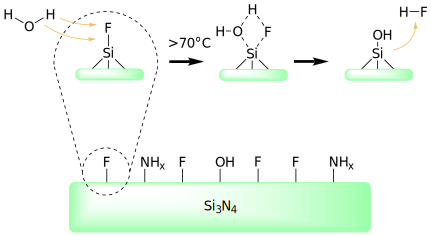
\includegraphics[width=1\linewidth]{Ressources/Chemistry/SiN}
	\capption{Proposed modification of \gls{sin} with \gls{hf}}{}
	\label{fig:chem:func:sin}
\end{wrapfigure}
One of the used substrates in this work is \gls{sin} as passivation layer above magnetic sensors as it has a significant better diffusion barrier against water or sodium ions and is chemically very inert. \cite{lit:chem:sin:surface} However, due to its complex crystal structure it is also difficult to modify by common chemicals and the exact surface composition still subject to scientific discussion. \cite{lit:chem:sin:etchingcontrol} Apart from cleaning the surface with piranha, few other modification methods have been reported, but only one suitable for the direct generation of \gls{hydroxyl} groups.

There, as depicted in \ref{fig:chem:func:sin}, the reaction \ch{Si-OH + HF <-> Si-F + H2O} takes place reversibly due to the coincidence that \ch{Si-O} and \ch{O-H} as well as \ch{Si-F} and \ch{H-F} bonds have similar binding energies and hence the forward and reverse reactions a low activation energy. After Le Chatelier's principle, a depletion of \gls{hf} in the bulk leads then to an increase in surficial hydroxyl groups. \cite{lit:chem:sin:SiFSiOH} In further works, it has been determined that an oxidation with a similar protocol based on aequous \gls{hf} yields a variable \gls{siloxane} coverage with \SI{37(17)}{\percent} of a monolayer, which nevertheless can be used for stable, covalent attachment of silanes.  Nominally the same surface coverages of silicon oxide and nitride surfaces could be achieved by ethoxy- and chlorosilanization. \cite{lit:chem:sin:surfacEtchingandMod} As shown by \citep{lit:chem:sin:silane}, the subsequent surfaces exhibit beneficial biological properties and can be modified by further standard procedures.


\subsubsection{Oxygen Plasma}
Apart from wet chemistry methods, the exposure of a surface to oxygen plasma yields \gls{hydroxyl} groups as well. In a plasma chamber, a low-pressure gas is irradiated by \si{\kilo\hertz} to \si{\mega\hertz} waves to excite and ionize its atoms. In consequence, the UV-radiation emitted by the gas can photolyse typical organic bonds and remove surface contaminations. Additionally, reactive oxygen species such as \ce{O2+}, \ce{O2-}, \ce{O3} or \ce{O} either oxidize the surface as well or bind dissociated components with low vapor pressure. During an evacuation in the process, these molecules are removed from the chamber intrinsically. \cite{lit:chem:plasma}  

\subsection{Silane Chemistry}

By the use of silane chemistry a surface is rendered organofunctional with alkoxysilane molecules. Since glass, silicon, alumina, titania, and quartz surfaces, as well as other metal oxide interfaces, are rich in hydroxyl groups, silanes are particularly useful for modifying these materials. \cite{lit:chem:silanizingGlass}\\The general formula for a silane coupling agent (Fig. \ref{fig:chem:trialkoxysilane}) typically shows the two classes of functionality. X is a hydrolyzable group typically alkoxy, acyloxy, halogen or amine.
\\\begin{wrapfigure}[9]{r}{.25\linewidth}
	\vspace{-0.7\baselineskip}
	\centering
	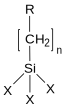
\includegraphics{Ressources/Chemistry/Trialkoxysilan}
	\capption{Trialkoxysilane}{Structure of a typical trialkoxysilane, X: hydrolyzable group, R: non-hydrolyzable organic radical, n: methylene chain-length}
	\label{fig:chem:trialkoxysilane}
\end{wrapfigure} 
Following hydrolysis, a reactive \gls{silanol} group is formed, which can condense with other silanol groups to form \gls{siloxane} linkages. 
(Fig. \ref{fig:chem:APTES}) Stable condensation products are also formed with other oxides such as those of aluminum, zirconium, tin, titanium, and nickel. Less stable bonds are formed with oxides of boron, iron, and carbon, whereas alkali metal oxides and carbonates do not form stable bonds with \glspl{siloxane} at all. The R group (Fig. \ref{fig:chem:trialkoxysilane}) is a nonhydrolyzable organic radical that may posses a functionality that imparts desired characteristics. One of the more common silanes is \gls{aptes}, where the X group consists of an \gls{ethoxy} group, the organic rest R is substituted by an \gls{amine} and the 3 \gls{methylene} groups alter \textit{n} to 3. \cite{lit:chem:GELEST} 
\begin{figure}[h]
	\centering
	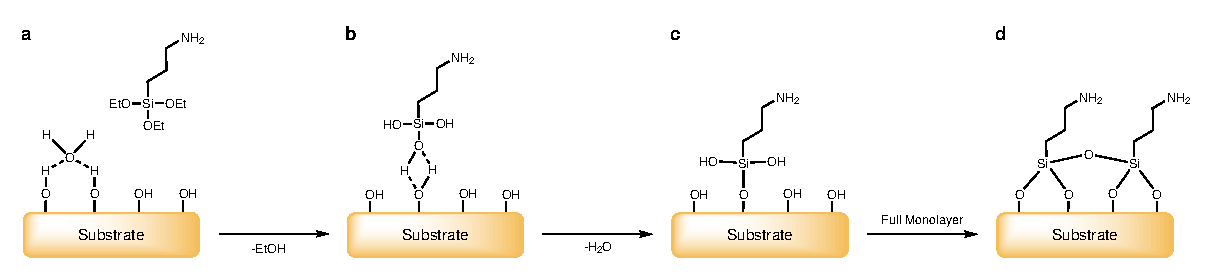
\includegraphics[width=1\linewidth]{./Ressources/Chemistry/APTES.eps}
	\capption{APTES Modifcation of an oxidized surface}{\textbf{a} Before the condensation reaction, the oxidized surface forms hydrogen bonds with water molecules. The silane molecules are in the bulk solution. \textbf{b} The hydrolyzed \gls{silanol} group adsorbs onto the surface and forms hydrogen bridges with it. \textbf{c} In a condensation reaction, under the loss of water, a covalent bond to the surface forms. \textbf{d} After the \gls{sam} assembly the surface is saturated with a covalent-bound, crosslinked silane film. \cite{lit:chem:aptes:SilaneReaction}}
	\label{fig:chem:APTES}
\end{figure}

The final result of reacting an organosilane with a substrate ranges from altering the wetting or adhesion characteristics of the substrate, utilizing the substrate to catalyze chemical transformation at the heterogeneous interface, ordering the interfacial region, and modifying its partition characteristics. Significantly, it includes the ability to effect a covalent bond between organic and inorganic materials. Especially in optical or biological sensors, silane modifications open a broad range of applications. 

However, the silanization reactions bear a few drawbacks which are often neglected. For instance, silane chemistry is strongly temperature and pH-dependent. \cite{lit:chem:silaizationTemp,lit:chem:silanizationParameters} Further, in a process to build \glspl{sam} out of \gls{aptes}, the reaction has to be catalyzed by water. But already small changes in the water content cause dramatic deviations in layer thickness. \cite{lit:chem:sin:selectivemod} Additionally, silanes can crosslink to themselves through possible side reactions. (Fig. \ref{fig:chem:APTES} D) \cite{lit:chem:aptes:Crosslink}



\subsection{Carbodiimide Crosslinker Chemistry}
The in previous manner produced \gls{amine}-terminated films by \gls{aptes} form the basis of many reactions and open the possibility to various applications, such as the direct attachment of biofunctional molecules by carbodiimide crosslinking chemistry.\cite{lit:bio:BioconjugateTechniques} Here, \gls{carboxyl} groups are modified by \gls{edc} and \gls{nhs} to form a stable secondary \gls{amide} bond with any primary \gls{amine}.

\begin{figure}[htb!]
	\centering
	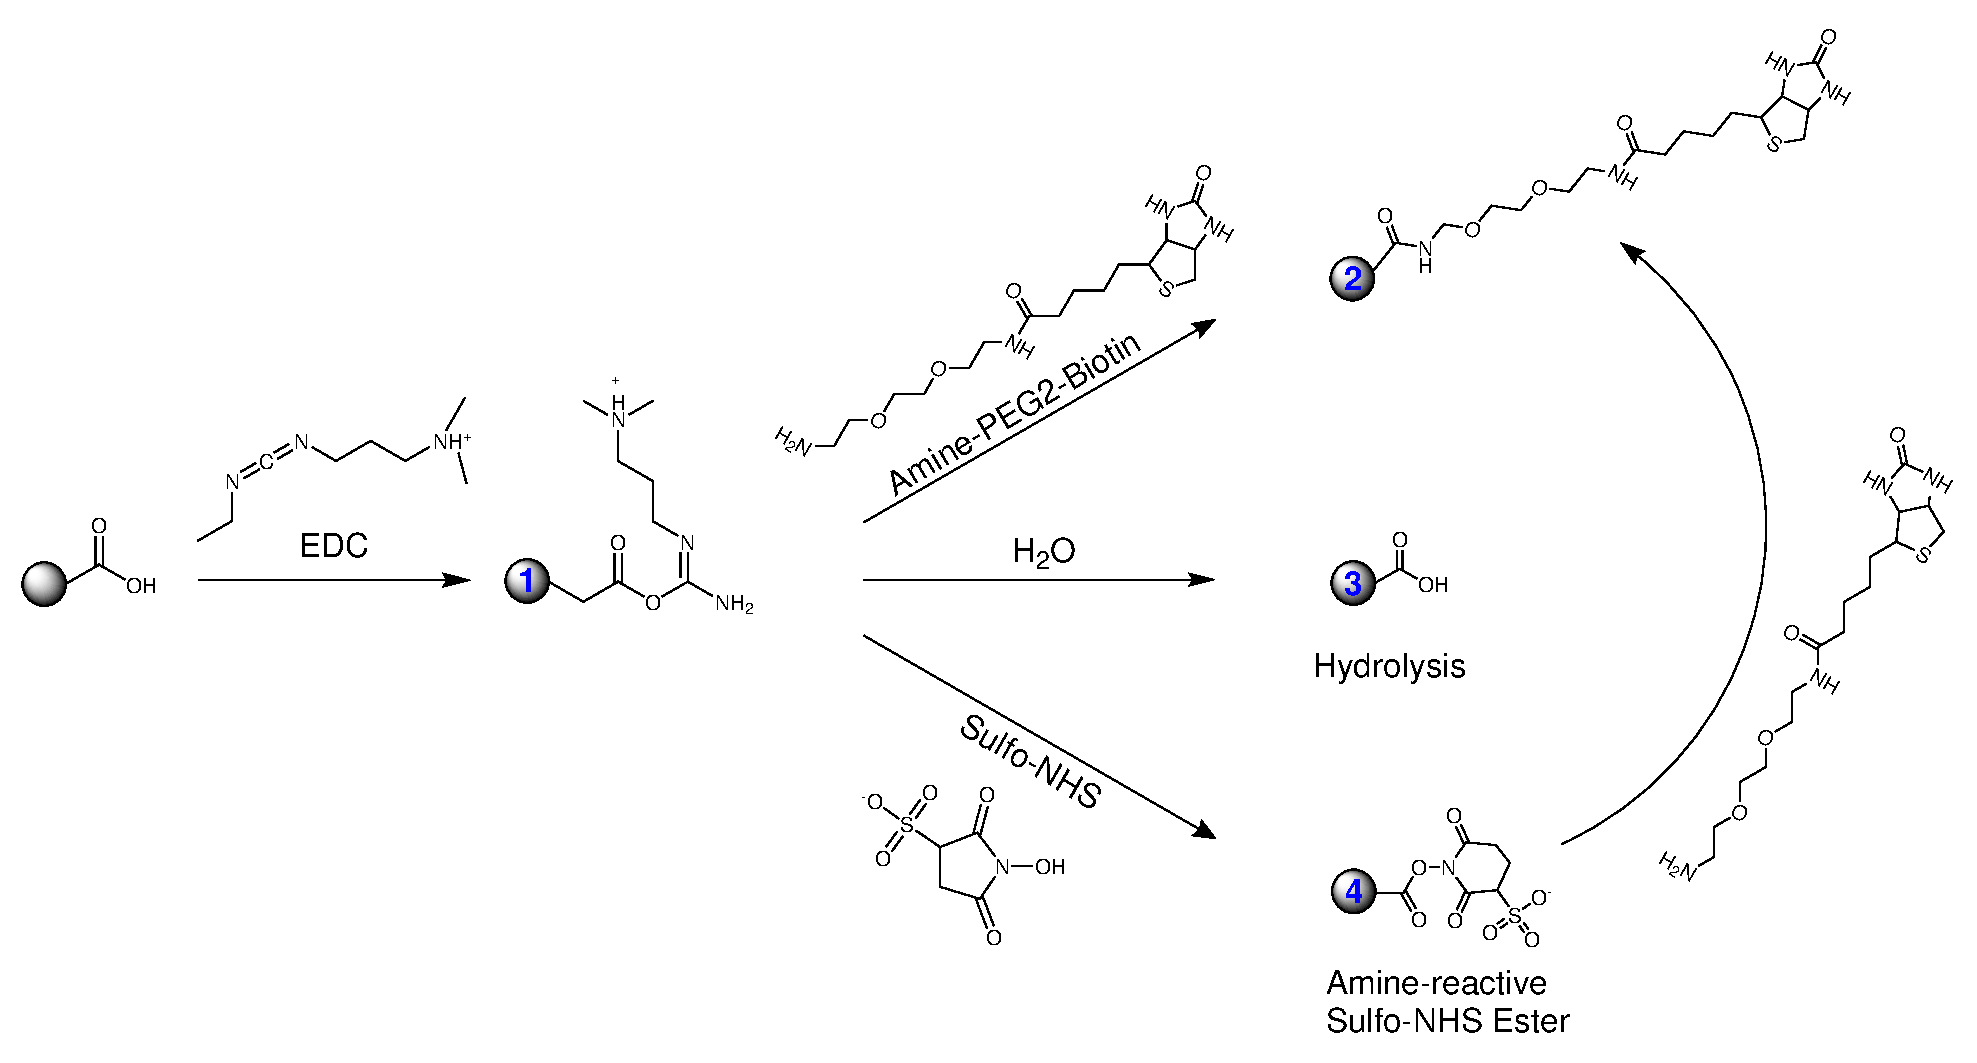
\includegraphics[width=\linewidth]{./Ressources/Chemistry/EDC-NHS.eps}
	\capption{Carboxyl bead modification with EDC/NHS}{The carboxy groups bead are activated with \gls{edc} to an active O-acylisourea intermediate. This can then either be nucleophilicly attacked by a primary amine of the amine-PEG$_2$-biotin reactant or - due to its instability - hydrolzed back to a regenerated carboxyl surface. A present NHS-ester can also displace the O-acylisourea to form a considerably more stable intermediate which then itself reacts with any primary amine.}
	\label{fig:chem:COOH-EDC-NHS}
\end{figure}
\clearpage
The general reaction mechanism is depicted in Fig. \ref{fig:chem:COOH-EDC-NHS} for the example of a microbead surface, but it can equivalently be applied to any other modified surface or molecule. The initial \gls{carboxyl} group is esterified by \gls{edc} to an active o-acylisourea intermediate and leaves rapidly upon nucleophilic attack of an amine with release of an iso-urea byproduct. A zero-length amide linkage is formed. (Fig. \ref{fig:chem:COOH-EDC-NHS}, 1->4) Sulfhydryl and hydroxyl groups also will react with such active esters, but the products of such reactions, thioesters and esters, are relatively unstable compared to an \gls{amide} bond. (Fig. \ref{fig:chem:COOH-EDC-NHS}, 1)\newline
However, this reactive complex is slow to react with amines and can hydrolyze in aqueous solutions, having a rate constant measured in seconds. If the target amine does not find the active \gls{carboxyl} before it hydrolyzes (Fig. \ref{fig:chem:COOH-EDC-NHS}, 3), the desired coupling cannot occur. This is especially a problem when the target molecule is in low concentration compared to water, as in the case of protein molecules. Notwithstanding, forming a \gls{nhs} ester intermediate from the reaction of the \gls{hydroxyl} group on NHS with the \gls{edc} active-ester complex increases the resultant amide bond formation remarkably. (Fig. \ref{fig:chem:COOH-EDC-NHS}, 3->4) \cite{lit:chem:nhs2}

Another critical point in carbodiimide chemistry is the solubility of the compounds. \gls{edc}, \gls{nhs} and \gls{snhs} are soluble in aqueous and organic solvents. Nevertheless, activation  with  non-sulfonate \gls{nhs} decreases water-solubility of the modified carboxylate molecule, while activation with \gls{snhs} preserves or increases its water-solubility by virtue of the charged sulfonate group. \cite{lit:chem:snhs}

\clearpage

\subsection{Microscopic Particle Surface Physics}
\todo{write!!!!}


\subsection{The Biotin-Avidin-System}
Until now, the interaction of the homotetrameric protein avidin and its ligand biotin forms one of the strongest known non-covalent bonds in biological systems characterized by a \gls{kd} in the range of \SI{e-15}{\molar}.\cite{lit:bio:biotin:avidin_discovery} First isolated from chicken egg white, it became a standard to use in biotechnology when researchers found a similar bacteria protein - streptavidin - in \textit{Streptomyces} strains.\cite{lit:bio:biotin:discovery} However, the charged glycoprotein avidin exhibits unspecific binding in some assays in comparison to streptavidin. Therefor, several companies developed deglycosylated forms of avidin with a neutral isoelectric points to minimize unspecificity. (NeutrAvidin, Extravidin, NeutraLite) In recent studies, a mutant streptavidin called ``Traptavidin'' exhibitied an even 10 times dissociation rate.\cite{lit:bio:biotin:engStrep}
As discovered in the early 1990s, biotin is bound inside a highly stable $\beta$-barrel structure, and stabilized by hydrogen bonds and van der Waals forces.\cite{lit:bio:biotin:bindingmechanism} In a unique mechanism, a side group of biotin (valerate) binds to a neighboring monomer of streptavidin and therefor stabilizes the dimer complex intrinsically.\cite{lit:bio:biotin:binding,lit:bio:biotin:freeenenergy} From a thermodynamical point-of-view, the interaction of the vitamin and protein is described by a total free binding energy of \SIrange{300}{330}{\kilo\joule\per\mole} for a tetrameric protein. \cite{lit:bio:biotin:freeenenergy}  All these aspects lead to a significant rupture force for the biotin-release of \SI{250}{\pico\newton}.\cite{lit:bio:biotin:rupture}

\begin{figure}[tbph!]
		\begin{subfigure}[b]{0.4\textwidth}
		\centering
		\addtocounter{subfigure}{1}  
		\subfigimg[height=150pt]{\textbf{a}}{./Ressources/Biology/biotin.eps}
		\addtocounter{subfigure}{-1}  
		\phantomsubcaption
		\label{fig:biotin}
	\end{subfigure}%
		\begin{subfigure}[b]{0.59\textwidth}
		\centering
		\addtocounter{subfigure}{1}  
		\subfigimg[clip, height=150pt]{b}{Ressources/Biology/crystalAvidin_bindingSite.png}		
		\addtocounter{subfigure}{-1}  
		\phantomsubcaption
		\label{fig:crystalavidin}
	\end{subfigure}%
	\capption{Functional Structures of Biotin and Streptavidin}{(\textbf{a}) Biotin chemical structure, (\textbf{b}) Homotetrameric Streptavidin with the anchor point at one terminus.\cite{lit:bio:SA:crystal}}
	\label{}
\end{figure}



\section{Magnetoresistive Sensing}
Short intro in GMR
Short intro over MRCyte


